\chapter{Nonlinear Optics}
\label{chap:2_nonlin_pol}
The model for nonlinear optical effects, as third harmonic generation, is already well-known in literature~\cite{Boyd2003}. However, in this Chapter we will describe the model for Harmonic Generation in a bulk material. Also, we shall look for the propagation of two waves coupled due to optical nonlinearity. This concepts shall be very useful to understand the dynamic of the generation of third harmonic in optical cavities.  

\section{Optical Polarization}
\label{sec:Optical_nonlinear}
An important subject of optical science to describe the interaction between light and matter is the existence of dipole moment per unit volume, which is called polarization. In a dielectric medium the polarization occurs mainly due to induced dipoles.

\begin{figure}[h!]
    \centering
    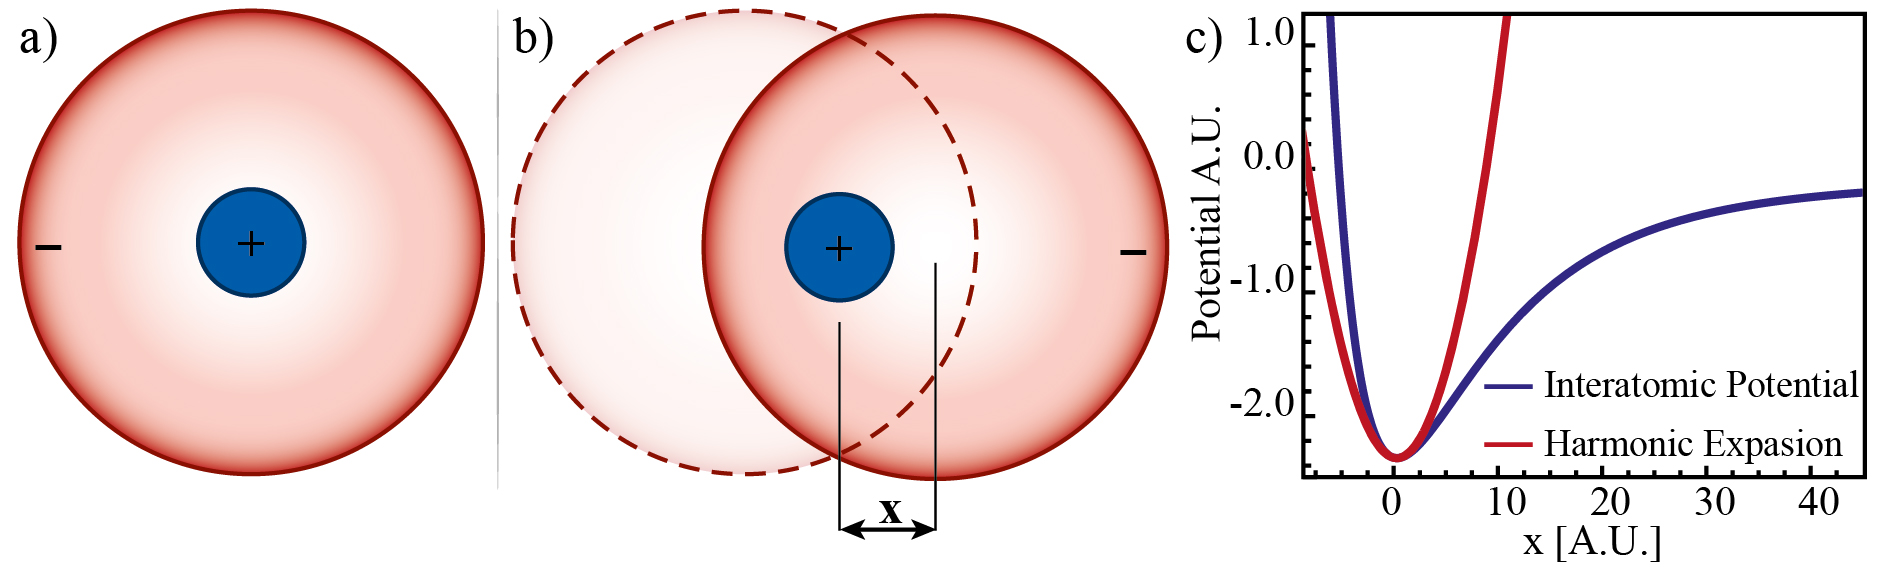
\includegraphics[width = 16cm]{figuras/Dissertation_atomic_polarization.jpg}
    \caption{\textbf{a) Atom in equilibrium:} the spherical symmetry of the atom makes it neutral for any external electric field. \textbf{b) Atom out of equilibrium:} If a strong enough external electric field are applied, it cause a displacement $x$ which generate a dipole with moment proportional on $x$. \textbf{c) Interatomic potential:} For a small displacement $x$ it is possible to approach the potential as an parable.}
    \label{fig:polarization}
\end{figure}
Lets consider a neutral atom placed in an external electric field $\vec{E}$. If the external electric field is negligible when compared with the internal electric field the initial equilibrium position is the concentric configuration, as shown in Fig.~\ref{fig:polarization}, this problem is analogous to the a solid spherical body charged with charge $q$ surrounded with a shell of charge $-q$. In a semiclasical approach we can consider all the charge concentrated in the center of each part~\cite{Griffiths2005}, which lead to a null total electric charge, hence to non electric field. However, the electron are free to move and thus the external electric field is able to displace the electron from the equilibrium position, creating a ionized dipole as shown in Fig.~\subref{fig:polarization}{b} (We consider that the external electric field isn't strong enough to deform the electronic cloud). It is easy to show that the dipole moment is proportional to displacement distance with the form~\cite{Griffiths2005}
\begin{equation}
    \vec{p} = q\vec{x}.
\end{equation}

When the external electric field is weak if compared with the interatomic electric field, we can approach the atomic potential to a parabolic, as show in Fig.~\ref{fig:polarization}c. The restoring force; therefore, is linear with distance. In such model, the polarization $\vec{p}$ is linear with the external electric field
\begin{equation}
    \vec{p} = \alpha \vec{E}.
\end{equation}
The constant $\alpha$ is called atomic polarization and depends on the atomic structure. This simple model is, in fact, in well agreement with experimental result.  

The result for a single atom can be easily extend for a solid body applying the principle of  superposition. In this way
\begin{equation}
    \vec{P} = \epsilon_0\chi^{(1)}\vec{E}.
\end{equation}
The information about the structure of the bulk material are contained in the constant $\susce{1}$; we call it linear electric susceptibility.

The assumption of weak external electric field implies in a small displacement, if compared with the atomic radius, otherwise we can't assume a parabolic potential due to the anharmonic form of the interatomic potential. 

In order to formulate a more general model, lets consider the motion of a electron in an anharmonic potential. Due to the spherical symmetry of the system, it is reasonable to assume that the motion of the electron occurs in the same direction on the applied electric field so we can avoid vectorial notation by define the generalized coordinate $x'$ in such way that the its real part is the displacement of the electron from the equilibrium position at this direction. We then have
\begin{equation}
    \ddot{x'} + 2\gamma\dot{x'} + \omega_0^2x'+ax'^2+bx'^3 = -eE(t)/m.
    \label{eq:motion_equation_electron}
\end{equation}
Here we assumed an applied time-dependent electric field given by $E(t)$, the electron charge as $-e$, a damping force of the form $-2m\gamma\dot{x'}$ and a restoring force given by
\begin{equation}
    F_\text{restoring} = -m\omega_0^2x' -max'^2 -mbx'^3, 
\end{equation}
where $a$ and $b$ are parameters that characterizes the strength of the nonlinearity. This restoring force corresponds to a potential energy with the form 
\begin{equation}
    U(x') = -\int F_\text{restoring} dx' = \frac{1}{2}m\omega_0^2x'^2 +\frac{1}{3}max'^3 +\frac{1}{4}mbx'^4.
\end{equation}

\begin{figure}[h!]
    \centering
    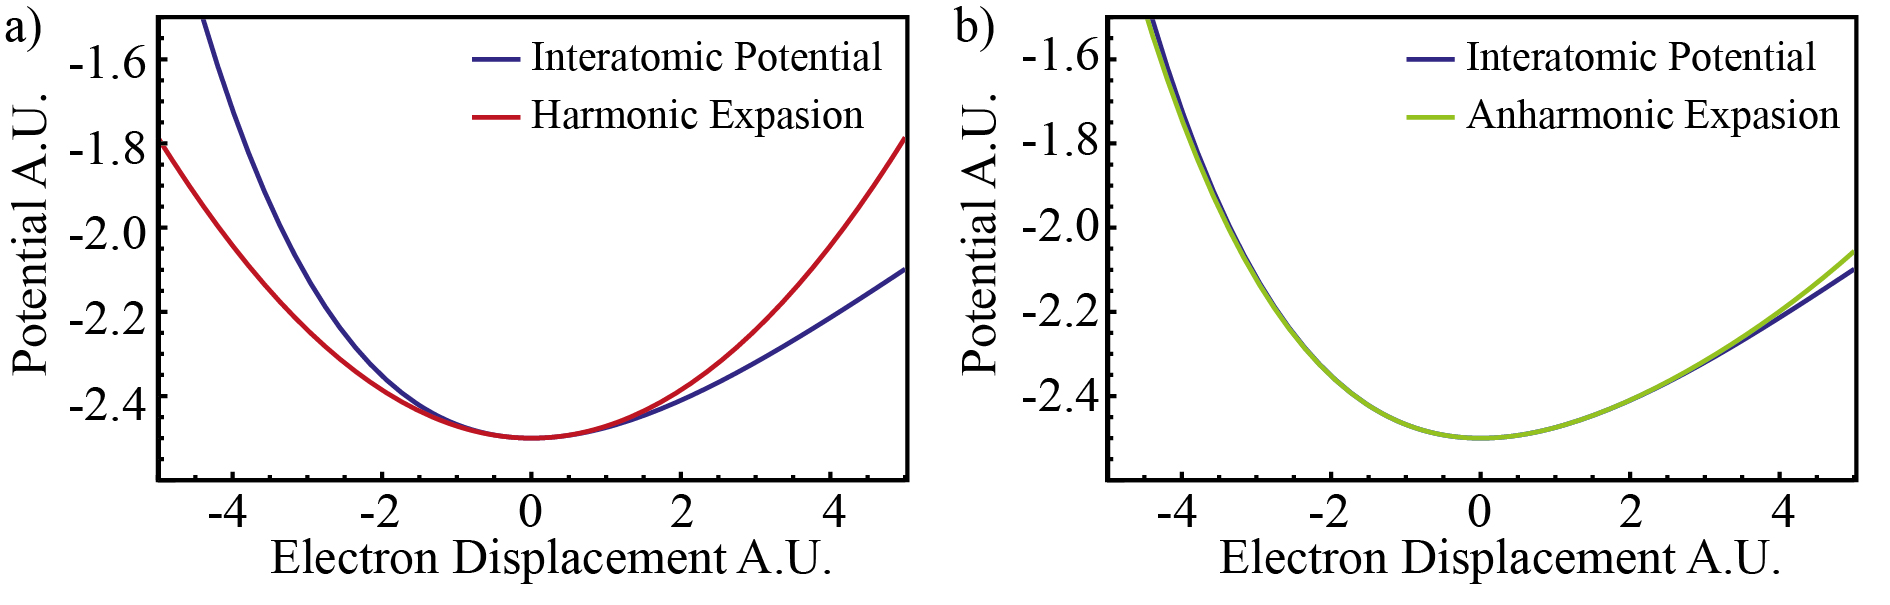
\includegraphics[width = 16cm]{figuras/Dissertation_interatomic_expassion.jpg}
    \caption{\textbf{a) Harmonic expansion:} The assumption of a parabolic potential are only valid if the Electron displacement are small when compared with the atom radius.\textbf{b) Anharmonic expansion:} Consider high order therms, anharmonic therms, for the expansion of the potential lead to a well agreement even when considered higher displacement.}
    \label{fig:expanssion}
\end{figure}
Eq.\ref{eq:motion_equation_electron} can be solved for using perturbation theory. Lets replace $E(t)$ by $\lambda E(t)$, %REWRITE: I must check Boyd calculus
\begin{equation}
    \ddot{x'} + 2\gamma\dot{x'} + \omega_0^2x'+ax'^2+bx'^3 = -\lambda eE(t)/m,
    \label{eq:pertubed_equation_electron}
\end{equation}
where $\lambda$ is continuous and ranges between zero and one. We seek for solutions in the form of power series of $\lambda$, that is 
\begin{equation}
    x' = \lambda x'^{(1)} + \lambda^2 x'^{(2)} + \lambda^3 x'^{(3)} +....
    \label{eq:x_pertubation_expanssion}
\end{equation}
This procedure give us a set of equations.
\begin{subequations}
    \begin{align}
        \ddot{x'}^{(1)} + 2\gamma\dot{x'}^{(1)} + \omega_0^2x'^{(1)} &= -eE(t)/m,\label{eq:first_order_pertubation}\\
        \ddot{x'}^{(2)} + 2\gamma\dot{x'}^{(2)} + \omega_0^2x'^{(2)}+a\left(x'^{(1)}\right)^2 &= 0,\label{eq:second_order_pertubation}\\
        \ddot{x'}^{(3)} + 2\gamma\dot{x'}^{(3)} + \omega_0^2x'^{(3)}+     2ax'^{(1)}x'^{(2)} +b\left(x'^{(1)}\right)^3 &= 0\label{eq:thirdt_order_pertubation}...    
    \end{align}
\end{subequations}

It is easy to see that the first order equation, Eq.~\ref{eq:first_order_pertubation}, is a problem of a forced harmonic oscillator. If considered a harmonic electric field with module $E(t) = Ee^{-i\omega t}$, for the steady-state we have
\begin{equation}
    x'^{(1)}(t) = \tilde{x}^{(1)}e^{-i\omega t}.
\end{equation}
The amplitude have the form
\begin{equation}
    \tilde{x}^{(1)} = -\frac{e}{m}\frac{E}{B(\omega)}.
\end{equation}
The function $B(\omega)$ are defined as $B(\omega) = \omega_0^2-\omega^2-2i\omega\gamma$.

Now we are able to rewrite Eq.~\ref{eq:second_order_pertubation} using the term in $x'^{(1)}$ as a driving force, which give us
\begin{equation}
    \ddot{x'}^{(2)} + 2\gamma\dot{x'}^{(2)} + \omega_0^2x'^{(2)} = a\left(\tilde{x}^{(1)}\right)^2e^{-i2\omega t}.
    \label{eq:second_order_motion_eq}
\end{equation}

Here we get a interesting result. Our system was initially drove by a harmonic force with frequency $\omega$, the anharmonicity of the interatomic potential bring forth a driven force with frequency $2\omega$. 

The steady-state solution of Eq.~\ref{eq:second_order_motion_eq} have the form
\begin{equation}
    x'^{(2)}(t) = \tilde{x}^{(2)}e^{-i2\omega t}.
\end{equation}
with the amplitude given by
\begin{equation}
    \tilde{x}^{(2)} = -\frac{a\left(eE\right)^2}{m^2B(\omega)^2B(2\omega)}.
\end{equation}

The same procedure for Eq.~\ref{eq:thirdt_order_pertubation} give us a perturbation with frequency $3\omega$, with the form 
\begin{equation}
    x'^{(3)}(t) = \tilde{x}^{(3)}e^{-i3\omega t},
\end{equation}
with amplitude
\begin{equation}
    \tilde{x}^{(3)} = -\frac{\left(eE\right)^3}{m^3B(\omega)^3B(3\omega)}\left(b+\frac{2a ^2}{B(2\omega)}\right).
\end{equation}

Eq.~\ref{eq:x_pertubation_expanssion} now give us a important insight. Even though the drive force due the external electric field is well defined with frequency $\omega$, the solution for the motion of the electron around the rest position gives us an harmonic series
\begin{equation}
    x'(t) = \lambda \tilde{x}^{(1)}e^{-i\omega t} + \lambda^2 \tilde{x}^{(2)}e^{-i2\omega t} + \lambda^3 \tilde{x}^{(3)}e^{-i3\omega t} +....
\end{equation}
Here we define the component drive by the external force as the fundamental mode of the motion of the electron and the high order terms are called second and third harmonic (later, we will apply this nomenclature for the optical mode).%REWRITE: I have defined nothing.  

This calculus can easily be extended to a vector analyse, along with the definition of dipole moment we can write
\begin{equation}
    \vec{p} = q\left(\lambda\vec{\tilde{x}}^{(1)}e^{-i\omega t}+\lambda^2\vec{\tilde{x}}^{(2)}e^{-i\omega t}+\lambda^3\vec{\tilde{x}}^{(3)}e^{-i\omega t}+... \right).
\end{equation}
For a bulk we have
\begin{equation}
    \vec{P} = \epsilon_0\chi^{(1)}\vec{E} + \epsilon_0\Bar{\chi}^{(2)}\vec{E}^2+\epsilon_0\Bar{\chi}^{(3)}\vec{E}^3+....
\label{eq:nonlim_pol}
\end{equation}
Note that the nonlinear susceptibility, $\Bar{\chi}^{(2)}$, $\Bar{\chi}^{(3)}$, are rank 2 and rank 4 tensors, respectively.

The main reason behind the math showed in this section is to make clear and intuitive that the generation of high orders harmonics occurs only due the interaction between an incident wave and the matter. This will be an important statement further below. 
%Now that I have convinced you that an anharmonic potential are able to generate high orders harmonic in the motion of the electrons leading to nonlinear terms for the polarization.% REWRITE.

\section{Wave Equation}
\label{sec:wave_equation}

We have looked on how the interaction between a harmonic wave electromagnetic wave and a nonlinear material generate high order harmonics. Lets now suppose the existence of two waves with different frequency and consider the effect of polarization upon the wave equation for a nonlinear optical medium~\cite{Boyd2003}. 

Starting with Maxwell's equations

\begin{subequations}
    \begin{alignat}{2}
        &\nabla\cdot\vec{D}  &&= 0,\\
        &\nabla\cdot\vec{B}  &&= 0,\\
        %\nabla\times\vec{E} &=  i \omega\vec{B}\\
        &\nabla\times\vec{E} &&= -\frac{\partial\vec{B}}{\partial t},\\ 
        %\nabla\times\vec{H} &= -i \omega\vec{D}\nabla\times\vec{E}
        &\nabla\times\vec{H} &&= \frac{\partial\vec{D}}{\partial t}.
    \end{alignat}
    \label{eq:max_eq}
\end{subequations}

We consider a nonmagnectic material, hence
\begin{equation}
    \vec{B} = \mu_0 \vec{H}
\end{equation}
%Otherwise, by consider a nonlinear medium, for the electric field we have
%\begin{equation}
%    \vec{D} = \epsilon_0\vec{E} + \vec{P}
%\end{equation}
%where $\vec{P}$ are given by Eq.~\ref{eq:nonlim_pol}.
%
In the absence of free charges and currents, we can then rewrite the Maxwell's equations in wave equation form for the electric field 
\begin{equation}
    \nabla^2\vec{E} - \frac{1}{\epsilon_0 c^2}\frac{\partial^2}{\partial t^2}\vec{D} = 0
\end{equation}
Finally, considering an nonmagnetic and nonlinear medium we can write the electric displacement field as
\begin{subequations}
    \begin{align}
        \vec{D} &= \epsilon_0\vec{E} +\vec{P},\\
        \vec{P} &= \vec{P}^{(1)} + \vec{P}^{(NL)}.
    \end{align}
\end{subequations}
In order to simplify the math, we split the polarization vector $\vec{P}$ in a linear part, given by $\vec{P}^{(1)} = \epsilon_0\chi^{(1)}\vec{E}$, and a nonlinear part $\vec{P}^{(NL)}$ given by all the remaining nonlinear terms of Eq.~\ref{eq:nonlim_pol}, so we have

\begin{equation}
    \nabla^2\vec{E} +\frac{\n^2}{c^2}\frac{\partial^2}{\partial t^2}\vec{E} = -\frac{1}{\epsilon_0 c^2} \frac{\partial^2}{\partial t^2}\vec{P}^{NL}.
    \label{eq:wave_equation_nonlinear}
\end{equation}
The refractive index, n, can be write as $\n^2= 1 + \chi^{(1)}$ and is a function of the frequency.

The following procedure can be applied for multiple nonlinear terms; however, since this is not the focus of this dissertation, we will proceed considering only the second order term. In such case

\begin{equation}
    \vec{P}^{NL} = \vec{P}^{(2)} = \epsilon_0\Bar{\chi}^{(2)}\vec{E}\vec{E}.
    \label{eq:nonlinear_polarization}
\end{equation}
%The total electric field is the sum of different frequency waves, for the second harmonic generation we have
Here, just for formality, was used explicitly the tensorial form of the nonlinear polarization and fields; however we will consider the case of a $z$ propagating wave in a isotropic medium, which enable us to use the nonlinear susceptibility as a scalar.

We are interested in the problem of how two different wave propagating in the same medium interact, wherefore the total electric field are the sum of this wave 
\begin{equation}
    \vec{E} = \vec{E}_1 + \vec{E}_2.
    \label{eq:total_field}
\end{equation}
The electric field of each wave can be write as    
\begin{equation}
    \vec{E}_\alpha = A_\alpha e^{i(k_\alpha z-\omega_\alpha t)}\hat{z} + c.c., \text{ for $\alpha = 1,2$}.
\end{equation}
As we saw in the Sec~\ref{sec:Optical_nonlinear}, the second order nonlinearity generate a wave with exactly twice the fundamental frequency, so $\omega_2 = 2\omega_1$. 

We are assuming that there is no other process beside second harmonic generation, resulting in a nonlinear polarization with two components, so that   
\begin{subequations}
    \begin{alignat}{1}
        \vec{P}^{(2)} &= \vec{P}^{(2)}_1+\vec{P}^{(2)}_2\\
        \vec{P}^{(2)}_\alpha &= P^{(2)}_\alpha e^{-i\omega_\alpha t}\hat{z}+c.c., \text{ for $\alpha$ = 1,2}.
    \end{alignat}
    \label{eq:nonlinear_polarization_harmonic_form}
\end{subequations}
%Due to the harmonic time dependence of the field, we can use $\frac{\partial}{\partial t} = -i\omega$, then Eq.~\ref{eq:wave_equation_nonlinear} can be write for each frequency, 

The left side of Eq.~\ref{eq:wave_equation_nonlinear} are composed by linear operators, we can write it as the sum of two equations. On the other hand, the left side of Eq.~\ref{eq:wave_equation_nonlinear} is, obviously, nonlinear which lead us to a system of two equation when arranging the therms with same harmonic the terms with the same time dependency  
\begin{subequations}
    \begin{alignat}{1}
        \frac{\partial^2}{\partial z^2}\vec{E}_1 +\frac{\omega_1^2}{c^2}\n_1^2 \vec{E}_1 = -\frac{\omega_1^2}{\epsilon_0 c^2} \vec{P}^{(2)}_1 \\
        \frac{\partial^2}{\partial z^2}\vec{E}_2 +\frac{\omega_2^2}{c^2}\n_2^2 \vec{E}_2 = -\frac{\omega_2^2}{\epsilon_0 c^2} \vec{P}^{(2)}_2
    \end{alignat}
\end{subequations}

Calculating Eq.~\ref{eq:nonlinear_polarization} and Eq.~\ref{eq:total_field}, comparing with Eq.~\ref{eq:nonlinear_polarization_harmonic_form} it is possible, and quit easy, to find that
\begin{subequations}
    \begin{align}
        P^{(2)}_1 &= 2\epsilon_0\chi^{(2)} A^*_1 A_2e^{i(k_2-k_1)z}\\
        P^{(2)}_2 &= \epsilon_0\chi^{(2)} {A_1}^2e^{i2k_1z}
    \end{align}
\end{subequations}


We can now analyze each frequency component, and simplify the equations by suppressing the vectorial notation. The full system of propagating wave equations are give by 
%\begin{subequations}
%    \begin{align}
%       \frac{\partial^2}{\partial z^2}A_1e^{ik_1z} +\frac{\omega_1^2}{c^2}\n_1^2 A_1e^{ik_1z} &= -2\frac{\omega_1^2 \chi^{(2)}}{\epsilon_0 c^2} A^*_1 A_2e^{-i\Delta kz}\\
%       \frac{\partial^2}{\partial z^2}A_2e^{ik_2z} +\frac{\omega_2^2}{c^2}\n_2^2 A_2e^{ik_2z} &= -\frac{\omega_2^2\chi^{(2)}}{\epsilon_0 c^2} A_1^2e^{i\Delta k z}
%    \end{align}
%\end{subequations}
\begin{subequations}
    \begin{align}
       \frac{\partial^2}{\partial z^2}A_1 +\frac{\omega_1^2}{c^2}\n_1^2 A_1 &= -2\frac{\omega_1^2 \chi^{(2)}}{c^2} A^*_1 A_2e^{-i\Delta kz}\\
       \frac{\partial^2}{\partial z^2}A_2 +\frac{\omega_2^2}{c^2}\n_2^2 A_2 &= -\frac{\omega_2^2\chi^{(2)}}{c^2} A_1^2e^{i\Delta k z}
    \end{align}
    \label{eq:coupled_wave_equation_SHC}
\end{subequations}
Here was defined the phase mismatch between the waves as
\begin{equation}
    \Delta k = 2k_1 - k_2.
\end{equation}

Eq.~\ref{eq:coupled_wave_equation_SHC} give us how the amplitude of the wave, especially the second harmonic, depends on the phase mismatch. 

Solution for coupled-wave equation have already been demonstrated; however, we are not interested in a analytic form for the amplitude, we ended up solving Eq.~\ref{eq:coupled_wave_equation_SHC} using numerical methods.

\begin{figure}[th!]
    \centering
    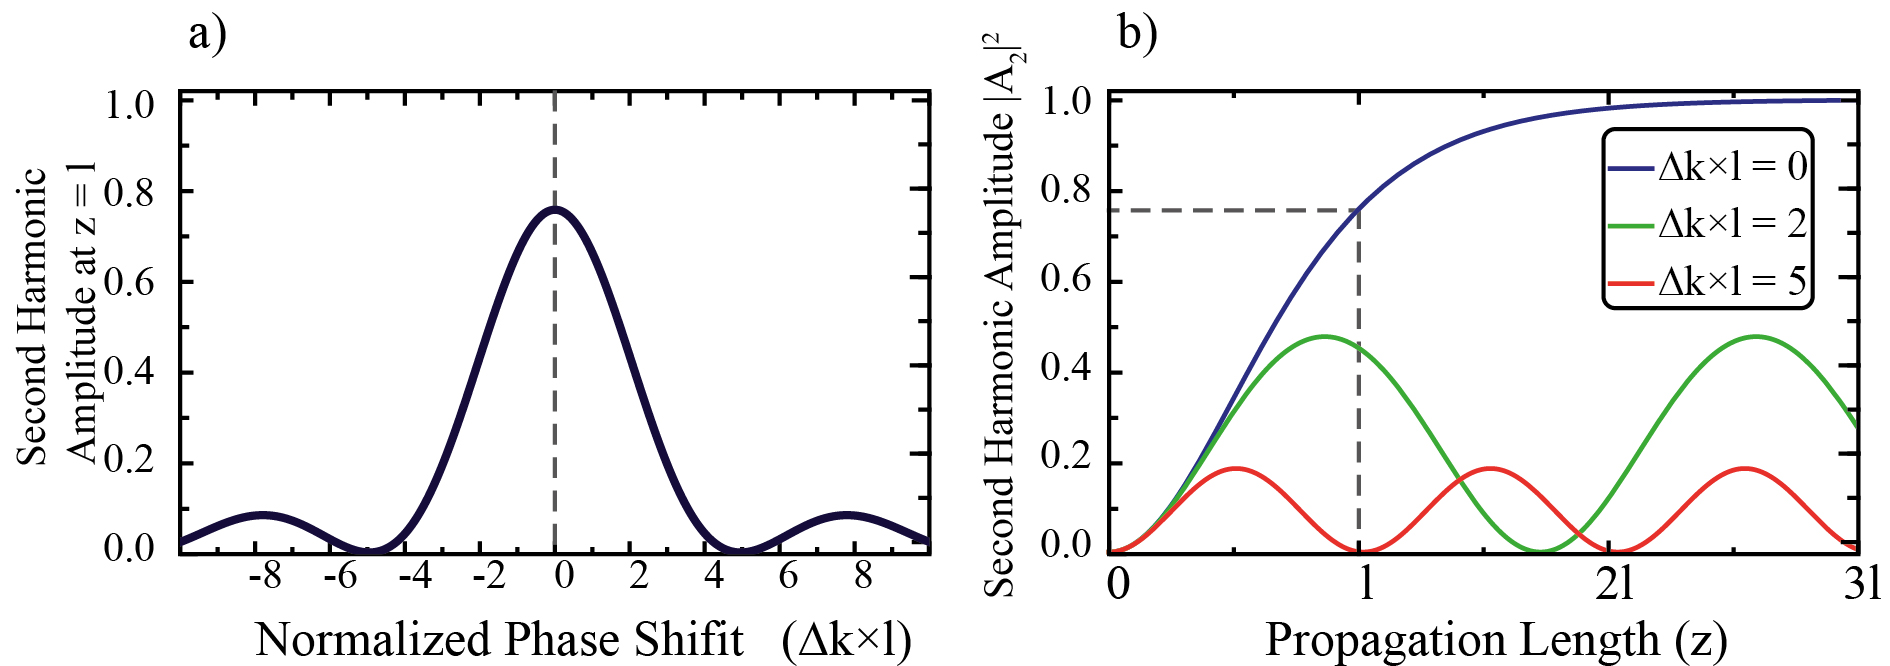
\includegraphics[width = 16cm]{figuras/Dissertation_coppled_eq_sol.jpg}
    \caption{\textbf{Coupled-wave equation numerical solution: a)} Modulus of the second harmonic amplitude, $|A_2|$, in function of $\Delta k \times l$ for $z = l$. \textbf{b)} Modulus of the second harmonic amplitude, $|A_2|$, in function of $z = l$ for different values of $\Delta k \times l$.}
    \label{fig:model_solution}
\end{figure}

In order to normalize the equations we define $l$ as the distance where, for $\Delta k = 0$, $75\%$ of the energy in the fundamental mode have been transferred for the second harmonic mode. 

Analysing the results presented in Fig.~\ref{fig:model_solution} it is possible observe two interesting, and indeed important, behaviors. Fig.~\subref{fig:model_solution}{a} shows that the amount of energy in the second harmonic model is maximum for $\Delta k = 0$; moreover, Fig.~\subref{fig:model_solution}{b} shows that the steady state are only reached for $\Delta k = 0$, any other value of $\Delta k$ lead to an oscillation as a function of the propagation distance.

\section{Conclusion}
Despite the focus of this project was not mathematically describe properties of material nor the propagation of coupled waves, we use this chapter to presents some quietly superficial math to reach two important conclusions.

First, we got from Sec~\ref{sec:Optical_nonlinear} that the wave generated due to second order nonlinearity presents exactly twice of the fundamental frequency, and this result come just from the interaction between the light and matter. 

Second, the Sec~\ref{sec:wave_equation} show us that an efficient conversion requires that the propagation of constant the second harmonic also to be double of the fundamental, otherwise we got a oscillatory dependence for the energy exchange and never reach a asymptote at the total conversion. 
% 
%
%However we got two, although obvious, important conclusion. First, was seen that the harmonic generation are result of the interaction between just the light and matter. Second, two modes are in phase matching only if both $\Delta \omega$ and $\Delta k$ are simultaneous zero.
%
Both conclusions will be better applied when we look for third harmonic generation in  modes confined in cavities. 

This result can be analogously make for third harmonic; however, it will give rinse for two additional terms responsible for a effect known as Kerr effect\cite{Barclay2005}. Due to third order nonlinearity the refractive index of the material change in amount proportional of the intensity of the electric field
\begin{equation}
    \text{n}(\omega_\alpha) = \text{n}_\alpha + \sum^{\beta=1,3} \text{n}_\beta |E_\beta|^2
    \label{eq:kerr_effect_free_wave}
\end{equation}

When considered, in typical laboratory condition, the Kerr effect includes a perturbation in the second term of the left side of Eq.~\ref{eq:wave_equation_nonlinear}. The following Chapter shall give us a more practical view of this effect.